\chapter{Decoding and Message Extraction}

This chapter describes how the data is decoded from the bit streams in order to extracting the message of the QR code. There is two key points which need to be clarified.
\begin{itemize}
\item The first one is we assume that we have the write QR code matrix based on the previous parts. Although some error might be tolerable(regarding the Reed-Solomon error correction) but still we need the QR-Matrix with not much errors.
\item The second one is that if the output message of this part is not correct that doesn't necessary mean that there is some mistakes in the previous parts.
\end{itemize}

The bit stream of the QR-Matrix is the item that connect the image processing part to the decoding part. If the software cannot reconstruct the QR pattern correctly then the decoding part of the software may not be able to decode the message. The flowchart of decoding/message extraction is as what can be seen in the next page.

The developed function $"decode\_ADVANCED\_QR"$, performs the task of decoding and message extraction.



\tikzstyle{decision} = [diamond, draw, fill=blue!20, 
    text width=4.5em, text badly centered, node distance=3cm, inner sep=0pt]
\tikzstyle{block} = [rectangle, draw, fill=blue!20, 
    text width=5em, text centered, rounded corners, minimum height=4em]
\tikzstyle{line} = [draw, -latex']
\tikzstyle{cloud} = [draw, ellipse,fill=red!20, node distance=3cm,
    minimum height=2em]
    
\begin{tikzpicture}[node distance = 3cm, auto]
    % Place nodes
    \node [cloud] (expert) {QR-Matrx};
    \node [block, below of=expert](init) {Decode Format Information};
    \node [cloud, right of=init, node distance=4cm] (system) {Version Num};
    \node [block, below of=init] (identify) {Demasking};
    \node [block, below of=identify] (evaluate) {Reed-Solomon Decoder};
    \node [block, left of=evaluate, node distance=4cm,text width=4cm] (update) {Detect/Correct errors};
    \node [decision, below of=evaluate, node distance=4cm] (decide) {is there any error?};
    \node [block, below of=decide, node distance=4cm,text width=4cm] (AP) {Decode Data Codewords and bit stream};
    \node [decision, right of=AP, node distance=5cm,text width=4cm] (FindAP) {Can you Detect Message Length and Encoding Mode?};
    
    \node [block, right of=FindAP, node distance=5cm] (Geo1) {Extract Final Message};
    \node [block, below of=FindAP, node distance=5cm,text width=4cm] (Geo2) {STOP/Double check Image Processing Part};
   % \node [block, above of=Geo1, node distance=3cm,text %width=4cm] (Crop) {Extract the QR-Code exact image};
 %   \node [block, above of=Crop, node distance=4cm,text %width=4cm] (FF) {Reed-Solomon Decoder/Message Extraction};
    % Draw edges
    \path [line] (init) -- (identify);
    \path [line] (identify) -- (evaluate);
    \path [line] (evaluate) -- (decide);
    \path [line] (decide) -| node [near start] {Yes} (update);
    \path [line,dashed] (update) -- (evaluate);
    \path [line] (decide) -- node {No}(AP);
    \path [line,dashed] (expert) -- (init);
    \path [line,dashed] (system) -- (init);
    \path [line,dashed] (system) |- (identify);
    \path [line] (AP) -- (FindAP);
    \path [line] (FindAP) -- node{Yes}(Geo1);
    \path [line] (FindAP) -- node{No}(Geo2);
    %\draw[ultra thick, blue, ->]  
    %(Geo1) -- (Crop);
    %\draw[ultra thick, blue, ->]  
    %(Geo2) -- (Crop);
    %\draw[ultra thick, red, ->]  
    %(Crop) -- (FF);

   
\end{tikzpicture}

\section{Decoding Data and Final Message}

In this section step by step, the process of decoding the final message will be described according to the previous flowchart. First the positions in the QR matrix which are related to data should be clarified. Using the following code first we put \textbf{"NaN"} in the non-data related positions.

\begin{lstlisting}
referenceIm = false(module);
referenceIm(1:8,1:8) = 1;       % left-upper corner(finder patters)
referenceIm(module-7:module, 1:8) = 1;    % left-down corner(finder patters)
referenceIm(1:8, module-7:module) = 1;    % right-upper corner(finder patters)
if module>21        % version 1 does not have alignment pattern
referenceIm(module-8:module-4,module-8:module-4) = 1;   % Alignment Pattern
end
 referenceIm(7,9:module-8) = 1;      % Horizontal Timing
 referenceIm(9:module-8,7) = 1;      % Vertical Timing
referenceIm(module-7,9) = 1;        % Dark module
\end{lstlisting}

Now we can deal with the other positions as "Data-Related bits".


\subsection{Version and QR code Matrix}

In this part the QR code Matrix and the version are the inputs. The version determines the number of modules in both directions. Since this project is about version 1 through 6 there is no version information in the QR matrix.

\subsection{Format Information Decoding}

In this step the format information which is placed in two
different locations inside the symbol have to be read. As we mentioned before in \ref{Format} there is two bits related to error correction level and three bits related to the number of mask pattern.

To decode the format information, the 15-bits format information should be XORed with the specific 15-bits which mentioned in \ref{Format}. But before XOR operation RS decoding has to be used for detecting and correcting the errors in that 15-bits string. After decoding, the first two bits and next three successive bits determine the error correction level and the number of mask pattern.

\subsection{Demasking}

According to the mask number calculated in the previous part, the matrix should be demasked before entering the Reed-Solomon decoder because in the generating procedure masking in after error correction coding.

\subsection{Reed-Solomon Decoding}

The error correction coding has been used to generate the QR code. Now using RS error correction decoder we need to detect and correct errors. For that first the bit stream should be converted to a decimal sequence to be used in Reed-Solomon decoder. RS decoder is an object which is provided within the "Communication Systems Toolbox" in MATLAB. Although it is provided by MATLAB but implementing it is not a trivial task. The script for Reed-Solomon decoding is as below:
\begin{lstlisting}
function [ str_decode ] = Reed_SLM_Decoder( msg,ECC )

m = 8; % Number of bits in each symbol
n = 2^m-1; k = n-length(ECC); % Codeword length and message length
hDec = comm.RSDecoder(n,k);
release(hDec)
hDec.GeneratorPolynomialSource = 'Property';
hDec.GeneratorPolynomial       = rsgenpoly(n,k,[],0);
c2 = [zeros(1,n-length(msg)-length(ECC)) msg ECC]';
d2 = step(hDec, c2);
d=d2(size(d2,1)-length(msg)+1:size(d2,1),1);
d=d';
str_decode=d;
end
\end{lstlisting}

Note that although RS codes are symmetric but we cannot use RS decoder directly because for the generation part there are different interleaving patterns for encoding the data and error correction codewords. refer to \cite{1iso} for more information.

\subsection{Message Extraction}

The corrected data codewords which have to be placed in the correct order should be converted in a binary bit stream. The first four bits indicate the mode that is used to
represent the codewords in bit sequence. Then the next 8 or 9 or  etc bits(depends on the encoding mode) demonstrate the message length. Finally by considering the procedure which mentioned in \ref{Encod} the message extraction should be done.

It is useful to demonstrate some results and final message of different test images to better following the results.


\begin{figure}[H]
     \begin{center}
%
        \subfigure[Verions-3 Qr code Message Extraction]{%
            \label{fig:first}
            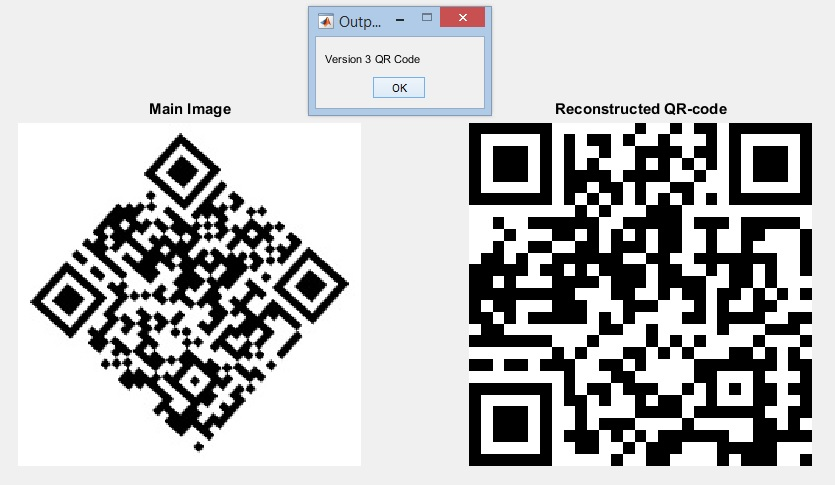
\includegraphics[width=0.9\textwidth]{figures/decod1.jpg}
        }\\%
        \subfigure[Verions-2 Qr High-resolution code]{%
           \label{fig:second}
           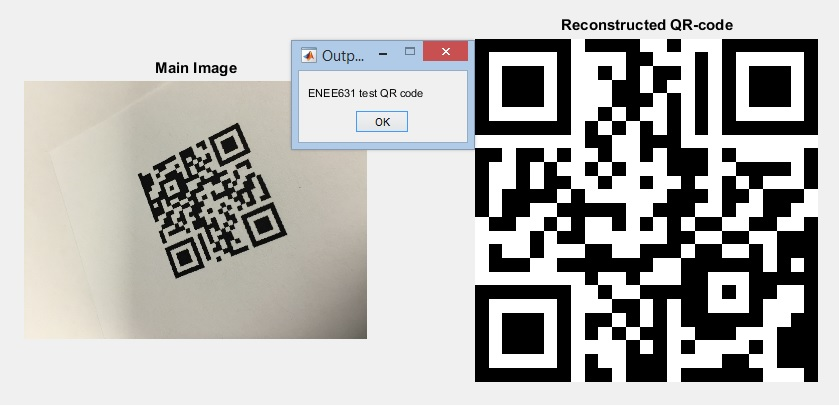
\includegraphics[width=0.9\textwidth]{figures/decod2.jpg}
        }\\%  ------- End of the first row 
        \subfigure[Verions-2 Qr code side view]{%
           \label{fig:second}
           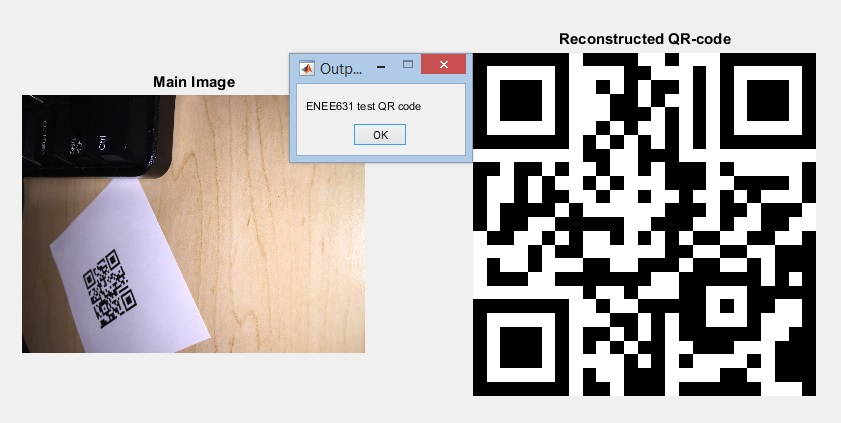
\includegraphics[width=0.9\textwidth]{figures/decod3.jpg}
        }
    \end{center}
    \caption{%
Message extraction of Version-2 and Version-3
     }%
   \label{fig4.1}
\end{figure}

\newpage
Now it is interesting to decode a QR doce from higher version. The following image is a version-5 QR code.

\begin{figure}[H]
  \caption{Version-5 QR code message extraction}
  \centering
    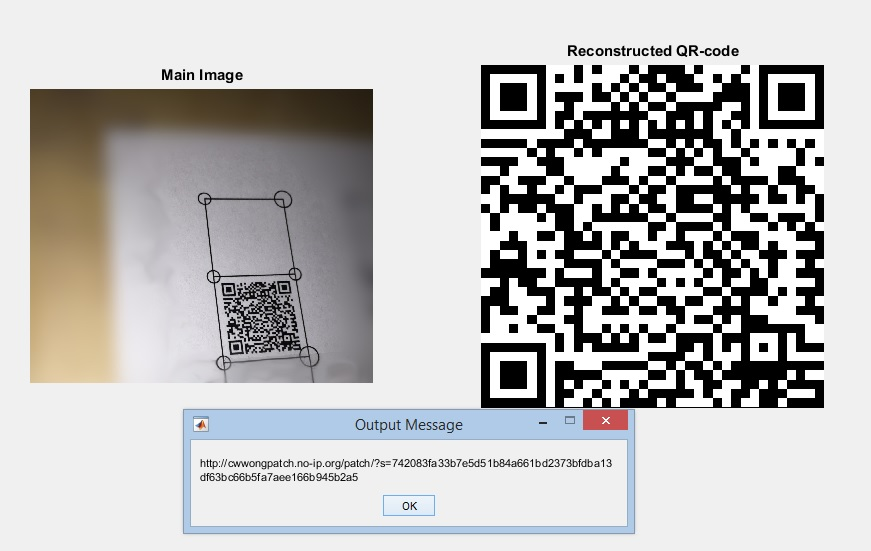
\includegraphics[width=0.9\textwidth]{figures/decod4.jpg}
    \label{fig:4.2}
\end{figure}

In this chapter the final part which is decoding and demonstrating the message has been described in detail and results were shown. Next chapter is the conclusion of the project and provides some discussions about the alternative approaches and deficiencies.
